% Section content template for individual Educative lessons
% This file contains the actual content for a specific section
% Generated from Educative API section content

% Section: Introduction to Pub-Sub
% Section ID: 5155663642099712
% Section Slug: introduction-to-pub-sub
% Generated: 2025-12-07T21:16:47.063533

Pub-sub messaging offers asynchronous communication. Let's explore the use cases where it is beneficial to have a pub-sub system.

\subsection{Use cases of pub-sub}\label{PIoWmcakwydMwkUWhwQHm}
\\
A few use cases of pub-sub are listed below:

\begin{itemize}
\item
\protect\phantomsection\label{P06FCjXhYFESKTrkpyO4t}
\textbf{Improved performance}: The pub-sub system enables push-based distribution, alleviating the need for message recipients to check for new information and changes regularly. It encourages faster response times and lowers the delivery latency.
\item
\protect\phantomsection\label{Rrf7I0iwO0ZVAKil49Iar}
\textbf{Handling ingestion}: The pub-sub helps in handling log ingestion(Log ingestion refers to importing logs into a database for immediate use, such as monitoring. Huge applications like Facebook produce massive amounts of data and logs. Real-time fetching and processing of logs allow us to run analysis and take quick actions in case of failures.). The user-interaction data can help us figure out useful analyses about the behavior of users. We can ingest a large amount of data to the pub-sub system, so much so that it can deliver the data to any analytical system to understand the behavior patterns of users. Moreover, we can also log the details of the event that's happening while completing a request from the user. Large services like Meta use a pub-sub system called Scribe to know exactly who needs what data, and remove or archive processed or unwanted data. Doing this is necessary to manage an enormous amount of data.
\item
\protect\phantomsection\label{mujHUKrDW1715GCoHyTFd}
\textbf{Real-time monitoring}: Raw or processed messages of an application or system can be provided to multiple applications to monitor a system in real time.
\item
\protect\phantomsection\label{Y_6ScBhi_v9ONeuqkqX94}
\textbf{Replicating data}: The pub-sub system can be used to distribute changes. For example, in a leader-follower protocol, the leader sends the changes to its followers via a pub-sub system. It allows followers to update their data asynchronously. The distributed caches can also refresh themselves by receiving the modifications asynchronously. Along the same lines, applications like WhatsApp that allow multiple views of the same conversation---for example, on a mobile phone and a computer's browser---can elegantly work using a pub-sub, where multiple views can act either as a publisher or a subscriber.
\end{itemize}

\begin{figure}[htbp]
 \centering
 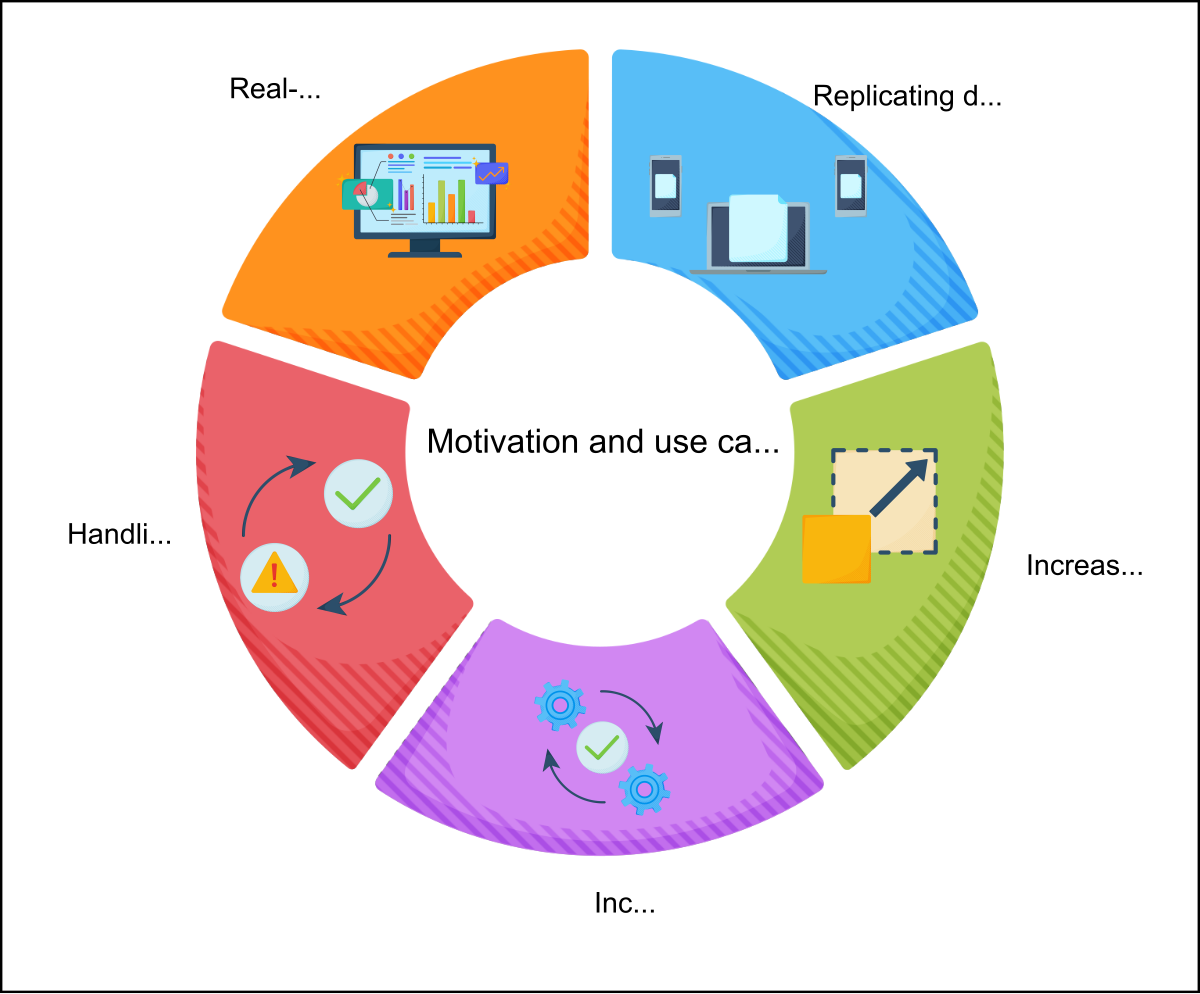
\includegraphics[width=0.5\textwidth]{Images/chapter_18/section_5155663642099712/5611026244829184.png}
 \caption{Motivation and use cases of the pub-sub system}
\end{figure}

\begin{quote}
\textbf{Quiz:}
\textbf{Question 1:} What are the similarities and differences between a pub-sub system and queues?
\textbf{Answer:} The pub-sub system and queues are similar because they deliver information that's produced by the producer to the consumer. The difference is that only one consumer consumes a message in the queue,

while there can be multiple consumers of the same message in a pub-sub system.
\textbf{Question 2:} How are producers and consumers decoupled from one another in a pub-sub system?
\textbf{Answer:} Producers don't know who'll end up reading their information. They just send it to the system, and it is read by the consumer. The system acts as a decoupling layer between the producers and consumers. Producers are not affected by slow consumers, the count of consumers, or the failure of consumers. We can scale them independently.
\end{quote}

\subsection{Requirements}\label{UZjUgXZvyZZmintq0wxxh}
\\
We aim to design a pub-sub system that has the following requirements.

\subsubsection{Functional requirements}\label{RaTSUulhCJhquZ9Zz2eqf}
\\
Let's specify the functional requirements of a pub-sub system:

\begin{itemize}
\item
\protect\phantomsection\label{3hs5-dXbuy0biNcy6yU6T}
\textbf{Create a} \textbf{topic}(A topic is a collection of related events or messages. The producers can create a topic and write the message into a topic. Consumers can subscribe to a topic and read from that topic.): The producer should be able to create a topic.
\item
\protect\phantomsection\label{xtcZyiVnp_Sqk3JRCYWXR}
\textbf{Write messages}: Producers should be able to write messages to the topic.
\item
\protect\phantomsection\label{UL_O8yQ41sP5U0fDnSAyP}
\textbf{Subscription}: Consumers should be able to subscribe to the topic to receive messages.
\item
\protect\phantomsection\label{_6ZoJaFuJ8RYp0G3RDbWe}
\textbf{Read messages}: The consumer should be able to read messages from the topic.
\item
\protect\phantomsection\label{KlwrmVLJNLji1JyzSgOjk}
\textbf{Specify retention time}: The consumers should be able to specify the retention time after which the message should be deleted from the system.
\item
\protect\phantomsection\label{oH9UTeM0xJsiPFRucndOE}
\textbf{Delete messages}: A message should be deleted from the topic or system after a certain retention period as defined by the user of the system.
\end{itemize}
\\
You're designing a real-time chat application that has channels for different discussions.~Explain how you would use a pub-sub system for its messaging component.~
\\
Describe the mapping of the chatting application onto the following pub-sub components:

\begin{itemize}
\item
Topics
\item
Subscribers
\item
How message delivery would work\\
\end{itemize}
\\
Write your answer in the widget below.

\textbf{Question:}

How you would use a pub-sub system in a chat application?

\textbf{Reference Answer:}

\begin{enumerate}
\def\labelenumi{\arabic{enumi}.}
\tightlist
\item
Topics: Channels.
\item
Subscribers: Users within the channel.
\item
Message delivery: Publishers (users sending messages) publish to their topic. The pub-sub brokers broadcast messages to all topic subscribers.
\end{enumerate}

\subsubsection{Non-functional requirements}\label{MS0cp2MxXhT_-yMhOTnKw}
\\
We consider the following non-functional requirements when designing a pub-sub system:

\begin{itemize}
\item
\protect\phantomsection\label{0uO49KA5R7nz6TzuAIQo_}
\textbf{Scalable}: The system should scale with an increasing number of topics and increasing writing (by producers) and reading (by consumers) load.
\item
\protect\phantomsection\label{pIh8croBsYd99oLavZAGO}
\textbf{Available}: The system should be highly available, so that producers can add their data and consumers can read data from it anytime.
\item
\protect\phantomsection\label{P2UeIW3fcwFrgFLuAZcGe}
\textbf{Durability}: The system should be durable. Messages accepted from producers must not be lost and should be delivered to the intended subscribers.
\item
\protect\phantomsection\label{3GKYTqMJBUj0Y98x5BTcD}
\textbf{Fault tolerance}: Our system should be able to operate in the event of failures.
\item
\protect\phantomsection\label{Fm6_Qr49YGa2atoh2jZvD}
\textbf{Concurrent}: The system should handle concurrency issues where reading and writing are performed simultaneously.
\end{itemize}

\subsection{API Design}\label{Sdd1SF3wedDpbMekDeBq1}
\\
We'll exclude some parameters from the functions below, such as the producer or consumer's identifier. Let 's assume that this information is available from the underlying connection context. The
API design for this problem is as follows:

\subsubsection{Create a topic}\label{YgfxpWLqYVQkRvfhKhOAM}
\\
The API call to create a topic should look like this:

\begin{verbatim}
create(topic_ID, topic_name)
\end{verbatim}

This function returns an acknowledgment if it successfully creates a topic, or an error if it fails to do so.

\begin{table}[htbp]
\centering
\small
\adjustbox{max width=\textwidth}{
\begin{tabular}{|p{0.275\textwidth}|p{0.675\textwidth}|}
\hline
\textbf{Parameter} & \textbf{Description} \\
\hline
\hline
\texttt{topic\_ID} & It uniquely identifies the topic. \\
\hline
\texttt{topic\_name} & It contains the name of the topic. \\
\hline
\end{tabular}
}
\end{table}

\subsubsection{Write a message}\label{iD1_czKzO7mi6mXs-OOkZ}
\\
The API call to write into the pub-sub system should look like this:

\begin{verbatim}
write(topic_ID, message)
\end{verbatim}

The API call will write a \texttt{message} into a topic with an ID of topic\_ID. Each message can have a maximum size of 1 MB. This function will return an acknowledgment if it successfully places the data in the systems, or an appropriate error if it fails.

\begin{table}[htbp]
\centering
\small
\adjustbox{max width=\textwidth}{
\begin{tabular}{|p{0.275\textwidth}|p{0.675\textwidth}|}
\hline
\textbf{Parameter} & \textbf{Description} \\
\hline
\hline
\texttt{message} & The message to be written in the system. \\
\hline
\end{tabular}
}
\end{table}

\subsubsection{Read a message}\label{EuM-YLbnZmAEPU4TJT5NW}
\\
The API call to read data from the system should look like this:

\begin{verbatim}
read(topic_ID)
\end{verbatim}

The topic is found using topic\_ID, and the call will return an object containing the message to the caller.

\begin{table}[htbp]
\centering
\small
\adjustbox{max width=\textwidth}{
\begin{tabular}{|p{0.259\textwidth}|p{0.691\textwidth}|}
\hline
\textbf{Parameter} & \textbf{Description} \\
\hline
\hline
\texttt{topic\_ID} & It is the ID of the topic against which the message will be read. \\
\hline
\end{tabular}
}
\end{table}

\subsubsection{Subscribe to a topic}\label{QRN3R4iFBE5nKTapz4AAB}
\\
The API call to subscribe to a topic from the system should look like this:

\begin{verbatim}
subscribe(topic_ID)
\end{verbatim}

The function adds the consumer as a subscriber to the topic that has the topic\_ID.

\begin{table}[htbp]
\centering
\small
\adjustbox{max width=\textwidth}{
\begin{tabular}{|p{0.259\textwidth}|p{0.691\textwidth}|}
\hline
\textbf{Parameter} & \textbf{Description} \\
\hline
\hline
\texttt{topic\_ID} & The ID of the topic to which the consumer will be subscribed. \\
\hline
\end{tabular}
}
\end{table}

\subsubsection{Unsubscribe from a topic}\label{ncOGTJOcQhSNqt0plo5ZL}
\\
The API call to unsubscribe from a topic from the system should look like this:

\begin{verbatim}
unsubscribe(topic_ID)
\end{verbatim}

The function removes the consumer as a subscriber from the topic that has the topic\_ID.

\begin{table}[htbp]
\centering
\small
\adjustbox{max width=\textwidth}{
\begin{tabular}{|p{0.259\textwidth}|p{0.691\textwidth}|}
\hline
\textbf{Parameter} & \textbf{Description} \\
\hline
\hline
\texttt{topic\_ID} & The ID of the topic against which the consumers will be unsubscribed. \\
\hline
\end{tabular}
}
\end{table}

\subsubsection{Delete a topic}\label{eHKKCJy20rMuuO5QlnO-o}
\\
The API call to delete a topic from the system should look like this:

\begin{verbatim}
delete_topic(topic_ID)
\end{verbatim}

The function deletes the topic on the basis of the topic\_ID.

\begin{table}[htbp]
\centering
\small
\adjustbox{max width=\textwidth}{
\begin{tabular}{|p{0.259\textwidth}|p{0.691\textwidth}|}
\hline
\textbf{Parameter} & \textbf{Description} \\
\hline
\hline
\texttt{topic\_ID} & The ID of the topic which is to be deleted. \\
\hline
\end{tabular}
}
\end{table}

\subsection{Building blocks we will use}\label{IKX-fjarmW4rDIidvUlgl}
\\
The design of pub-sub utilizes many building blocks that have been discussed in the initial chapters. We 'll consider the following lessons on building blocks.

\begin{figure}[htbp]
 \centering
 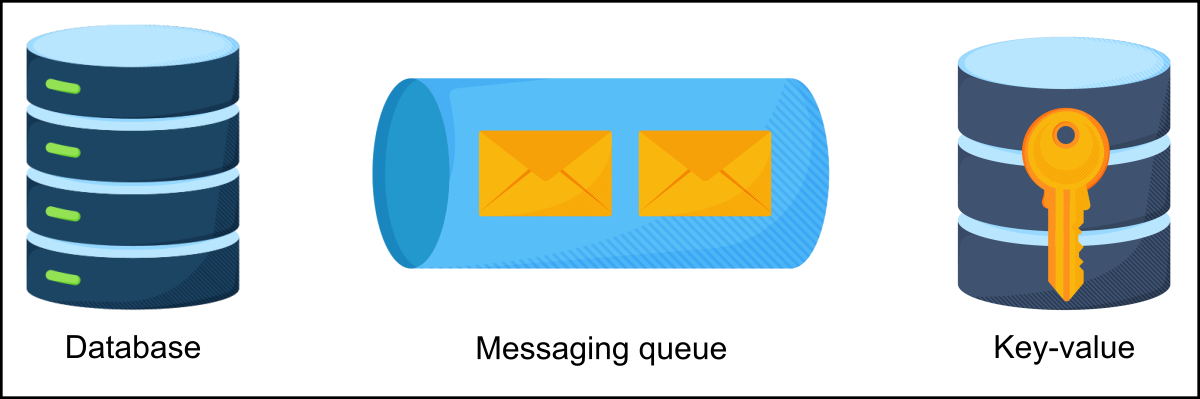
\includegraphics[width=0.5\textwidth]{Images/chapter_18/section_5155663642099712/6561638906200064.png}
 \caption{The building blocks we’ll use}
\end{figure}

\begin{verbatim}
create(topic_ID, topic_name)
\end{verbatim}

\begin{itemize}
\item
\protect\phantomsection\label{VvJl3tPArMHwmIzLzmG-f}
\href{https://www.educative.io/courses/grokking-the-system-design-interview/introduction-to-databases}{\textbf{Database}}: We'll use databases to store information like subscription details.
\item
\protect\phantomsection\label{8vhL8LPM0l5FsCkbteXZP}
\href{https://www.educative.io/courses/grokking-the-system-design-interview/system-design-the-distributed-messaging-queue}{\textbf{Distributed messaging queue}}: We'll use a messaging queue to store messages sent by the producer.
\item
\protect\phantomsection\label{8Q-ymqobQpjlPpcS9pQFj}
\href{https://www.educative.io/courses/grokking-the-system-design-interview/system-design-the-key-value-store}{\textbf{Key-value}}: We'll use a key-value store to hold information about consumers.
\end{itemize}
\\
In the next lesson, we'll focus on designing a pub-sub system.

% End of section content